\chapter{L'approccio proposto}
\section{Identificazione automatica di clienti con comportamenti atipici}

L’identificazione dei clienti che stanno effettuando delle transazioni fraudolente è il tema centrale dell'antiriciclaggio. Al fine di individuare queste persone, durante il progetto di stage è stato deciso di identificarli attraverso un approccio basato sull'individuazione di comportamenti anomali nelle loro transazioni.
Il fine del progetto è quello di sviluppare un algoritmo non supervisionato che identifichi, in modo automatico, tutti quei soggetti che hanno un comportamento anomalo rispetto a tutti gli altri appartenenti alla stessa banca.

Per l'identificazione di tutti quei comportamenti da segnalare come anomali l'approccio è stato basato sul clustering, ovvero sul raggruppare in cluster soggetti con
comportamenti simili tramite l'osservazione delle loro transazioni nell'arco
temporale di un mese, tutti i clienti che non andavano ad inserirsi in uno dei cluster
venivano successivamente posti sotto osservazione.

Tuttavia un solo discostamento dal cluster non è una motivazione sufficiente per segnalare un soggetto come fraudolento, tale movimento può essere avvenuto a causa di particolari festività oppure a causa di un evento imprevisto nella vita del cliente.
Per questo motivo ogni cliente viene monitorato per vari mesi e se questo comportamento si ripete per un numero di volte fissato viene deciso di segnalarlo.

Il discostarsi da un cluster, quindi avere un comportamento differente rispetto a tutti gli altri clienti della banca non è l'unico comportamento che viene tenuto sotto controllo nel monitoraggio di possibili comportamenti fraudolenti.
Infatti, un altro segnale di riciclaggio, è lo spostamento frequente da un cluster ad un altro di un cliente, infatti un comportamento normale di un cliente dovrebbe essere quello di muoversi all'interno del cluster con piccole variazioni dovute a normali eventi esterni.

La finalità del progetto è stato quindi quello di creare un algoritmo che analizzasse le transazioni di ogni cliente all'interno di un singolo mese, quindi su un intervallo di trenta giorni, analizzando attraverso differenti variabili descrittive il loro comportamento soffermandoci principalmente sul loro comportamento rispetto ai cluster: variavano spesso cluster o diventavano punti isolati senza mai essere riassorbiti.
Quando questi comportamenti atipici si ripetono più volte nel tempo parte quindi la segnalazione.



\section{Le principali variabili descrittive}

Per identificare i comportamenti fraudolenti dei clienti, vengono selezionate diverse variabili descrittive che incrociate fra loro producano evidenze di ciò che è oggetto del progetto:
\begin{itemize}
\item Numero di operazioni totali effettuate da una singola persona in un mese
\item Numero di operazioni totali di incremento del conto corrente
\item Numero di operazioni totali di decremento del conto corrente
\item Numero di giorni in cui sono state effettuate operazioni di incremento del conto corrente
\item Numero di giorni in cui sono state effettuate operazioni di decremento del conto corrente
\item Numero di giorni in cui sono state effettuate operazioni sia di incremento che di decremento del conto corrente
\item Numero totale di giorni in cui sono state effettuate operazioni di qualsiasi genere
\item Importo totale movimentato da operazioni di qualsiasi tipi in un mese
\item Importo totale movimentato in operazioni di incremento in un mese
\item Importo totale movimentato in operazioni di decremento in un mese
\item Transazione minima 
\item Transazione massima 
\item Saldo medio di ogni cliente 
\item Saldo minimo di ogni cliente 
\item Saldo massimo di ogni cliente 
\item Saldo finale di ogni cliente 
\end{itemize}


\section{Clustering mensile e anomalie ``statiche"}
Tramite l'ausilio delle variabili precedentemente introdotte sono state monitorate delle configurazioni di transazioni che potevano risultare appartenere ad una  possibile frode nel ambito del riciclaggio di denaro.
L'approccio che è stato deciso di proporre si compone di una parte \textit{statica}, ovvero di un analisi focalizzata su ciò che avviene in un determinato lasso di tempo senza compararlo con ciò che è avvenuto prima o dopo, ed è quella che andiamo ad analizzare in questo paragrafo, ed una \textit{dinamica} che analizzeremo nel paragrafo successivo.

Nel nostro caso il periodo di tempo considerato è stato un mese, con cui si intende un mese di calendario (es. Febbraio, Marzo...) e non un periodo di 30 giorni, questo perché lavorando con una banca è di più facile estrazione un mese con questa accezione. In aggiunta, nel momento in cui una frode dovesse essere segnalata sarà più facile il recupero delle transazioni in un mese predefinito, rispetto ad periodo di tempo da noi scelto arbitrariamente.

Effettuiamo quindi un clustering mensile, presi tutti i clienti che in quel mese hanno effettuato operazioni, tramite un clustering di tipo gerarchico sono stati formati dei cluster dell'intera popolazione di clienti della banca. 

L'analisi è stata condotta producendo anche degli scatterplot per poter analizzare in modo visivo la composizione dei cluster e renderne la comprensione più semplice per gli operatori che in seguito andranno a visionare gli eventuali clienti segnalati come possibili fraudolenti.
Questa facilità di visualizzazione è data dalla colorazione differente che ogni cluster possiede rendendo più semplice individuare l'appartenenza di un componente ad un determinato cluster.

\begin{figure}[H]
    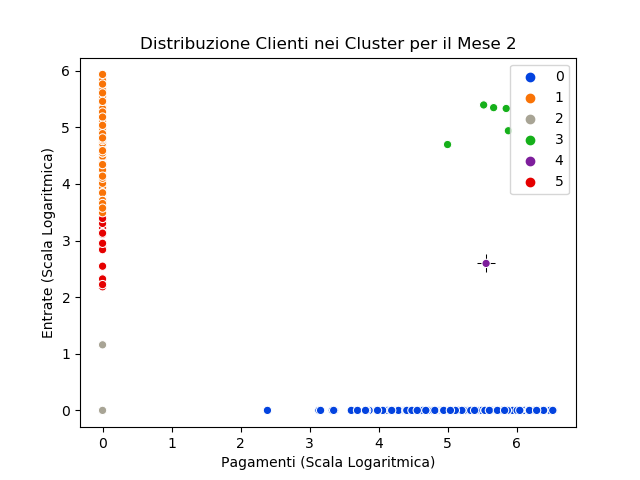
\includegraphics[width=0.9\textwidth]{M2.png}
    \centering
    \caption{Scatterplot di esempio}
    \label{fig:esScatter}
\end{figure}

Quando dalla scomposizione degli utenti in cluster viene rilevato che un utente forma un cluster singolo, ovvero in cui l’unico componente è lui e non sono presenti altri clienti, viene segnalato come anomalo sollevando un \textit{alert} su di lui.

Nel momento in cui un utente è l’unico componente di un cluster significa che ha avuto un comportamento anomalo rispetto a tutti gli altri clienti della banca in quel mese, viene quindi segnalato anche nel caso in cui sia la prima volta che questo accade. La segnalazione non equivale ad affermare che quella persona stia effettuando una frode, ma piuttosto a porla sotto osservazione per andare ad analizzare se quel comportamento è un avvenimento isolato oppure è parte di uno schema di riciclaggio di denaro.
Nel caso in cui dovesse risultare da un analisi longitudinale che questa persona è risultata anomala per vari mesi allora il livello di attenzione a cui è sottoposto incrementerebbe e si aggiungerebbe il flag di possibile persona fraudolenta.

Durante l'analisi è stato deciso di non soffermarsi solo sulla particolarità di formare cluster singoli ed essere quindi etichettati come un anomalia, ma è stato deciso di approfondire l'analisi di questa particolarità andando ad individuare delle \textit{regole} ovvero delle spiegazioni delle anomalie che questi utenti hanno prodotto attraverso i loro movimenti.

Queste regole, una volta che questi utenti sono riconosciuti come realmente fraudolenti, possono essere impiegate in AML come schema conosciuto di riciclaggio e riconoscere in minor tempo future frodi e prevenirle.

Per definire le \textit{regole} che caratterizzano un cliente, o più clienti, con comportamento anomalo all'interno di un mese è stato, come prima cosa, identificato il numero di cluster formati dai clienti in quel mese e il numero di componenti di ognuno. Il numero di cluster si è reso necessario perché il setting sperimentale (basato su dati reali) su cui è stato testato il nostro approccio è molto esiguo e in alcuni mesi comprendeva un solo utente oppure un solo cluster a cui appartenevano tutti i clienti. Un altra casistica che poteva accadere, a causa della quale il mese doveva essere scartato, era la presenza di più cluster ma tutti con un numero di utenti maggiore di uno.
Durante questa fase vengono inoltre creati degli scatterplot per vedere anche in modo grafico i cluster formati dai clienti in quel mese come in figura \ref{fig:esScatter}.

Nel momento in cui sono stati identificati i mesi in cui era presente un cluster formato da una sola persona, solitamente molto distante anche graficamente da tutti gli altri, ci si è andati a concentrare su ogni singolo mese andando a segnalare il cliente potenzialmente fraudolento.
Il dataset iniziale in cui comparivano tutte le transazioni aggregate e riassunte di quel mese è stato quindi arricchito di una colonna \textit{Fraud} che valeva 0 nel caso in cui quel utente non fosse segnalato come fraudolento e 1 nel caso in cui avesse formato un cluster singolo e quindi fosse da tenere sotto osservazione.
Questo dataset così composto è stato dato in input ad un \textit{Decision Tree Classifier }per andare ad estrarre le regole, intese come spiegazione dell'anomalia riscontrata, per il particolare cliente. 

Queste regole così estratte esprimono il comportamento del cliente e sono facilmente riconducibili al posizionamento dei punti sullo scatterplot (ognuno corrispondete ad un cliente) che vengono creati durante la fase di clustering, i risultati ottenuti da queste verranno discussi nei capitoli successivi. 

\section{Analisi longitudinale dei clusters e anomalie ``dinamiche"}

L’approccio che è stato deciso di proporre per l’identificazione di persone che attuano schemi di riciclaggio si compone di una parte \textit{statica}, descritta nel paragrafo precedente e una parte \textit{dinamica} che trattiamo in questo paragrafo.

Un anomalia \textit{dinamica} è un anomalia che viene identificata comparando tra loro i dati e le analisi relative a più mesi, possiamo associarla ad un cliente che presenta varie anomalie statiche nei mesi dell'orizzonte temporale considerato oppure ad un cliente che non è mai risultato anomalo ma ha effettuato un salto di cluster nell'ultimo mese.

L’analisi delle anomalie statiche di un mese produce come risultato una tabella in cui ogni identificativo (ID) di ogni utente è associato al cluster in cui si è trovato in quel mese ed eventualmente se è risultato anomalo. Partendo dalle tabelle così ottenute per tutto l’orizzonte temporale considerato andiamo a delineare le anomalie dinamiche. I dati contenuti in queste permettono di individuare se questo utente è stato già anomalo precedentemente nel periodo temporale considerato e quante volte lo è stato. Il numero di volte che questo è accaduto determina l’innalzare il livello di allerta di possibile comportamento fraudolento per quel utente, la \textit{regola statica} che viene fornita come spiegazione del comportamento sarà quella prodotta nell'ultimo mese in cui l'utente è stato anomalo.

Tuttavia, se l’utente non è mai risultato anomalo nel periodo considerato ma \textit{salta} ovvero cambia cluster vi sono delle considerazioni differenti da fare.

Le possibili motivazione alla base del cambio di cluster di un utente possono essere molteplici, una fra tutte il cambio di abitudini e quindi di profilo dell'utente. Lo spostamento frequente fra i cluster potrebbe comunque essere un segnale di comportamento fraudolento e necessita di segnalazione. 

Bisogna però tenere in considerazione la possibilità che i cluster si modifichino durante i mesi, unendosi o dividendosi in modo spontaneo, in questo caso non si tratterebbe di un vero e proprio salto, per questo motivo andiamo a considerare le sotto popolazioni all'interno di un cluster per mantenere una consistenza dei cluster tra i mesi.
Preso il cluster al mese precedente a quello considerato si va ad analizzare la composizione di esso e allo stesso modo si verifica la composizione del cluster a cui appartiene l’utente nel mese considerato, per questo motivo è di fondamentale importanza tenere traccia dei cluster a cui sono appartenuti i clienti in ogni mese.

Se nel cluster è presente una sotto popolazione del cluster del mese precedente allora l'utente non ha effettuato un salto di cluster, ma bensì si è mosso in maniera coerente rispetto alla sua sotto popolazione, non va quindi a rappresentare un anomalia.

Nel caso in cui il cluster del mese considerato non contenga nessun utente già presente nel cluster di cui faceva parte il cliente nel mese precedente, siamo di fronte ad un salto di cluster anomalo e come tale viene segnalato tramite un alert, se questo comportamento dovesse reiterarsi nel tempo è un segnale di possibile frode e il livello di attenzione su quel utente andrebbe ad incrementare.
Consideriamo anomalo quando è un solo cliente a saltare, quando invece sono almeno due il cambio di cluster potrebbe essere dovuto a motivi fiscali o legislativi e nel nostro caso non lo consideriamo anomalo.

Partendo quindi dalle anomalie statiche di ogni cliente e dalle regole che le descrivono, si segnalano nei mesi precedenti i clienti che sono risultati anomali tramite: il numero di mesi della finestra temporale in cui è stato sollevato un alert oppure dalla percentuale di segnalazioni rispetto al totale di transazioni di un utente.

Tutti questi dati raccolti vengono raccolti in una tabella riassuntiva finale che contiene: ogni utente con il proprio identificativo (ID), la motivazione ovvero la regola che abbiamo estratto in precedenza che spiega l'anomalia e il periodo temporale in cui sono stati rilevati come fraudolenti. L’operatore a cui questi dati sono destinati andrà quindi a valutare le transazioni del utente o degli utenti segnalati per capire se effettivamente siamo nel caso di transazioni finalizzate al riciclaggio di denaro oppure a movimenti legittimi. 



\section{Progettazione del prototipo, ambiente software e librerie utilizzati}

Durante il progetto di stage è stato sviluppato un prototipo come conclusione e sintesi dell'approccio \textit{statico} proposto e per permettere una più facile interpretazione per gli operatori finali. Il prototipo (chiamato in seguito anche \textit{demo}) prende in input i dataset relativi al periodo temporale di cui si vuole analizzare la scomposizione in cluster ed eventualmente, se presente, sottolineare una possibile anomalia statica. 
Per ogni mese del periodo temporale viene eseguito il clustering gerarchico e individuati i cluster ed il relativo numero di componenti, nel caso in cui all'interno del mese fossero presenti degli utenti con comportamento anomalo associabile ad un anomalia statica vengono evidenziati, come si può vedere nell'immagine \ref{fig:mese1}. Inoltre tramite dei barplot viene esplicitato la numerosità dei clienti fraudolenti in quel mese.

\begin{figure}[H]
    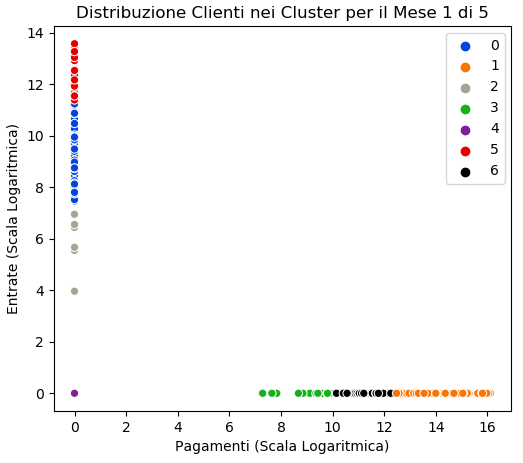
\includegraphics[width=0.8\textwidth]{Clustering_Mese_1.png}
    \centering
    \caption{Mese privo di clienti anomali}
    \label{fig:mese1}
\end{figure}
\begin{figure}[H]
    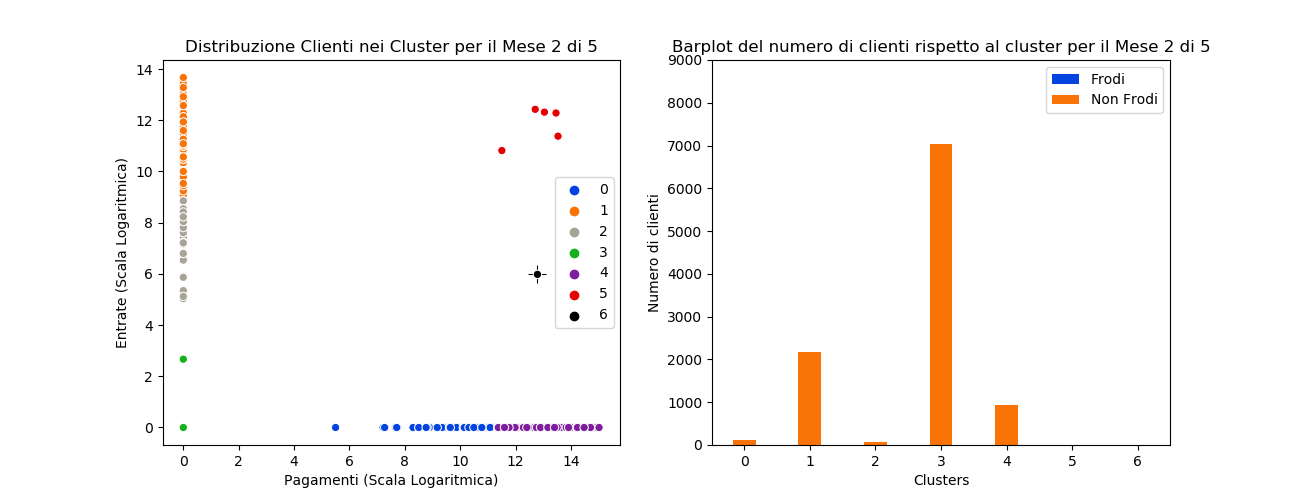
\includegraphics[width=1\textwidth]{Clustering_Mese_2.png}
    \centering
    \caption{Mese con un cliente anomalo}
\end{figure}


La demo è stata sviluppata in \textit{Python}, essendo il linguaggio utilizzato durante lo studio dell'approccio precedentemente descritto e la pre-elaborazione dei dati. \\ La piccola demo risultate è stata fornita come eseguibile al cliente per dare un primo sguardo su ciò che il progetto di stage arriverà ad essere. 


Per lo sviluppo della demo abbiamo impiegato le seguenti librerie:
\begin{itemize}
\item \textbf{Sklearn}\footnote{\url{https://scikit-learn.org/stable/index.html} in particolare Agglomerative Clustering } che fornisce supporto per molteplici algoritmi di machine learning, supervisionato e non supervisionato. 
\item \textbf{Seaborn}\footnote{\url{https://seaborn.pydata.org}}  per costruire grafici statistici in Python in particolare per la realizzazione di scatterplot e bar plot.
\end{itemize}


 %Nella nostra demo abbiamo utilizzato \textit{AgglomerativeClustering} per andare a creare i cluster mensili fondamentali per l'analisi delle anomalie statiche.
